\documentclass[tikz,border=2pt]{standalone}
\usepackage{amsmath,amssymb}
\usepackage{tikz}

\begin{document}
% A binary variable may take only the two values 0 (no) and 1 (yes); the continuous bounds
% 0 <= y <= 1 alone would allow every value in between.
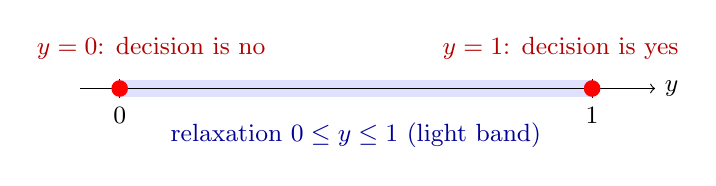
\begin{tikzpicture}[every node/.style={font=\small}]
	\draw[line width=6pt, blue!12] (0,0) -- (6,0);
	\draw[->] (-0.5,0) -- (6.8,0) node[right] {$y$};
	\foreach \x/\l in {0/0, 6/1} {\draw (\x,0.12) -- (\x,-0.12) node[below] {$\l$};}
	\fill[red] (0,0) circle (3pt); \fill[red] (6,0) circle (3pt);
	\node[red!70!black, anchor=south] at (0.4,0.25) {$y=0$: decision is no};
	\node[red!70!black, anchor=south] at (5.6,0.25) {$y=1$: decision is yes};
	\node[blue!60!black] at (3,-0.6) {relaxation $0\le y\le1$ (light band)};
	\end{tikzpicture}
\end{document}
